\section{Graphs}
\subsection{Introduction}

\begin{frame}{Graphs}{Introduction}
  \textbf{Graphs - Overview:}
  \begin{itemize}
    \item<2->
      Besides arrays, lists and trees the most common datastructure\\
      (Trees are a special type of graph)
    \item<3->
      Representation of graphs in the computer
    \item<4->
      Breadth first search (BFS)
    \item<5->
      Depth first search (DFS)
    \item<6->
      Connected components of a graph
  \end{itemize}
\end{frame}        

\begin{frame}{Graphs}{Introduction}
  \textbf{Terminology:}
  \onslide<2->
  \begin{columns}
    \begin{column}[b]{0.5\linewidth}
      \begin{figure}
        \begin{adjustbox}{width=0.75\linewidth}
          \begin{tikzpicture}[
  vertice/.style={
    circle,
    draw=Mittel-Blau,
    color=Mittel-Blau,
    inner sep=0em,
    minimum size=1.75em,
    line width=0.1em,
    font=\large
  }, edge/.style={
    draw={Mittel-Gruen},
    line width=0.2em
  }, edge_arrow/.style={
    edge,
    ->
  }
]%
\draw (0.0, 0.0) node[vertice] (vert0) {0};
\draw (2.0, 0.0) node[vertice] (vert1) {1};
\draw (4.0, -0.75) node[vertice] (vert2) {2};
\draw (1.5, -1.0) node[vertice] (vert3) {3};
\draw (-1.0, -1.5) node[vertice] (vert4) {4};

\draw[edge] (vert0) to (vert1);
\draw[edge] (vert1) to (vert2);
\draw[edge] (vert1) to (vert3);
\draw[edge] (vert2) to (vert3);
\draw[edge] (vert3) to (vert4);
\end{tikzpicture}%
        \end{adjustbox}
        %\caption{Undirected graph}
        \label{fig:graphs:introduction_undirected}
      \end{figure}
    \end{column}
    \begin{column}[b]{0.5\linewidth}
      \begin{figure}
        \begin{adjustbox}{width=0.75\linewidth}
          \begin{tikzpicture}[
  vertice/.style={
    circle,
    draw=Mittel-Blau,
    color=Mittel-Blau,
    inner sep=0em,
    minimum size=1.75em,
    line width=0.1em,
    font=\large
  }, edge/.style={
    draw={Mittel-Gruen},
    line width=0.2em
  }, edge_arrow/.style={
    edge,
    ->
  }
]%
\draw (0.0, 0.0) node[vertice] (vert0) {0};
\draw (1.5, -0.5) node[vertice] (vert1) {1};
\draw (4.0, -1.5) node[vertice] (vert2) {2};
\draw (1.5, -2.0) node[vertice] (vert3) {3};
\draw (4.5, 0.5) node[vertice] (vert4) {4};

\draw[edge_arrow] (vert0) to (vert1);
\draw[edge_arrow] (vert0) to (vert3);
\draw[edge_arrow] (vert1) to (vert2);
\draw[edge_arrow, bend left=15] (vert1) to (vert4);
\draw[edge_arrow] (vert2) to (vert3);
\draw[edge_arrow] (vert2) to (vert4);
\draw[edge_arrow] (vert3) to (vert1);
\draw[edge_arrow, bend left=15] (vert4) to (vert1);
\draw[edge_arrow, out=0, in=270, looseness=5] (vert2.east) to (vert2.south);
\end{tikzpicture}%
        \end{adjustbox}
        \vspace{-1.0em}
        %\caption{Directed graph}
        \label{fig:graphs:introduction_directed}
      \end{figure}
    \end{column}
  \end{columns}
  \begin{itemize}
    \item<3->
      Each Graph {\color{Mittel-Blau}$G = (V, E)$} consists of:
      \begin{itemize}
        \item<4->
          A set of vertices (nodes){\color{Mittel-Blau}$V = \{v_1, v_2, \dotsc\}$}
        \item<5->
          A set of edges (arcs) {\color{Mittel-Blau}$E = \{e_1, e_2, \dotsc\}$}
       \end{itemize}
     \item<6->
       Each edge connects two vertices
       ({\color{Mittel-Blau}$u, v \in V$})
       \begin{itemize}
         \item<7->
           Undirected edge: {\color{Mittel-Blau}$e = \{u, v\}$} (set)
         \item<8->
           Directed edge: {\color{Mittel-Blau}$e = (u, v)$} (tuple)
        \end{itemize}
      \item<9->
        Self-loops are also possible:
        {\color{Mittel-Blau}$e = (u, u)$} or
        {\color{Mittel-Blau}$e = \{u, u\}$}
  \end{itemize}
\end{frame}

%-------------------------------------------------------------------------------

\begin{frame}{Graphs}{Introduction}
  \textbf{Weighted graph:}
  \onslide<2->
  \begin{figure}
    \begin{adjustbox}{width=0.75\linewidth}
      \begin{tikzpicture}[
  vertice/.style={
    circle,
    draw=Mittel-Blau,
    color=Mittel-Blau,
    inner sep=0em,
    minimum size=1.75em,
    line width=0.1em,
    font=\large
  }, edge/.style={
    draw=Mittel-Gruen,
    line width=0.2em
  }, edge_arrow/.style={
    edge,
    ->
  }, edge_cost/.style={
    midway,
    color=Hell-Gruen,
    font=\Large
  }
]%
\draw (-2.0, -1.0) node[vertice] (vert0) {0};
\draw (1.5, -0.5) node[vertice] (vert1) {1};
\draw (6.0, -1.5) node[vertice] (vert2) {2};
\draw (1.5, -2.5) node[vertice] (vert3) {3};
\draw (4.5, 1.5) node[vertice] (vert4) {4};

\draw[edge_arrow] (vert0) to node[edge_cost, above] {3} (vert1);
\draw[edge_arrow] (vert0) to node[edge_cost, above] {2} (vert3);
\draw[edge_arrow] (vert1) to node[edge_cost, above] {2} (vert2);
\draw[edge_arrow, bend left=10] (vert1) to  node[edge_cost, above] {1} (vert4);
\draw[edge_arrow, bend right=10] (vert2) to node[edge_cost, above] {1} (vert3);
\draw[edge_arrow] (vert2) to node[edge_cost, right] {4} (vert4);
\draw[edge_arrow] (vert3) to node[edge_cost, right] {9} (vert1);
\draw[edge_arrow, bend right=10] (vert3) to node[edge_cost, below] {1} (vert2);
\draw[edge_arrow, bend left=10]
  (vert4) to node[edge_cost, below] {5} (vert1);
\draw[edge_arrow, out=0, in=270, looseness=5]
  (vert2.east) to node[edge_cost, below] {2} (vert2.south);
\end{tikzpicture}%
    \end{adjustbox}
    %\caption{Weighted graph}
    \label{fig:graphs:introduction_weighted}
  \end{figure}
  \begin{itemize}
    \item<3->
      Each edge is marked with a real number named {\color{Mittel-Blau}weight}
    \item<4->
      The {\color{Mittel-Blau}weight} is also named {\color{Mittel-Blau}length}
      or {\color{Mittel-Blau}cost} of the edge depending on the application
  \end{itemize}
\end{frame}

%-------------------------------------------------------------------------------

\begin{frame}{Graphs}{Introduction}
  \begin{columns}
    \begin{column}{0.40\linewidth}
      \textbf{Example:} Road network
      \begin{itemize}
        \item<2->
          Intersections: {\color{Mittel-Blau}vertices}
        \item<3->
          Roads: {\color{Mittel-Blau}edges}
        \item<4->
          Travel time:\\
          {\color{Mittel-Blau}costs of the edges}
      \end{itemize}
    \end{column}
    \onslide<5->
    \begin{column}{0.6\linewidth}
      \begin{figure}[!h]
        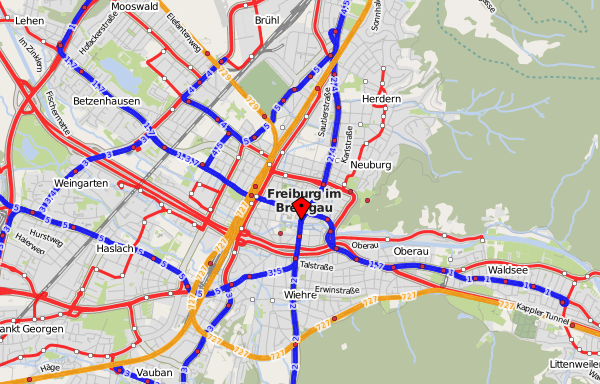
\includegraphics[width=\linewidth]
          {Images/Graphs/Freiburg_OpenStreetMap.png}
        \caption{Map of Freiburg $\copyright$~OpenStreetMap}
        \label{fig:graphs:introduction_freiburg_osm}
      \end{figure}
    \end{column}
  \end{columns}
\end{frame}


%-------------------------------------------------------------------------------

\subsection{Implementation}

\begin{frame}{Graphs}{Implementation}
  \textbf{How to represent this graph computationally?}
  \begin{itemize}
    \item<2->
      Two classic variants
    \begin{enumerate}
    \item<3->
      {\color{Mittel-Blau}Adjacency matrix} with space consumption
      \begin{math}
        \color{Mittel-Blau}
        \Theta(\vert V \vert^2)
      \end{math}
      \end{enumerate}
  \end{itemize}
  \onslide<4->
  \begin{columns}
    \begin{column}{0.45\linewidth}
      \begin{figure}[!h]
        \begin{adjustbox}{width=0.75\linewidth}
          \begin{tikzpicture}[
  vertice/.style={
    circle,
    draw=Mittel-Blau,
    color=Mittel-Blau,
    inner sep=0em,
    minimum size=1.75em,
    line width=0.1em,
    font=\large
  }, edge/.style={
    draw=Mittel-Gruen,
    line width=0.2em
  }, edge_arrow/.style={
    edge,
    ->
  }, edge_cost/.style={
    midway,
    color=Hell-Gruen,
    font=\Large
  }
]%
\draw (0.0, 0.0) node[vertice] (vert0) {0};
\draw (5.0, 0.25) node[vertice] (vert1) {1};
\draw (4.0, -3.0) node[vertice] (vert2) {2};
\draw (0.0, -3.5) node[vertice] (vert3) {3};

\draw[edge_arrow] (vert0) to node[edge_cost, above] {2} (vert1);
\draw[edge_arrow] (vert0) to node[edge_cost, right] {3} (vert3);
\draw[edge_arrow] (vert1) to node[edge_cost, right] {9} (vert2);
\draw[edge_arrow, bend right=15] (vert2) to node[edge_cost, above] {-1} (vert3);
\draw[edge_arrow] (vert3) to node[edge_cost, above] {7} (vert1);
\draw[edge_arrow, bend right=15] (vert3) to node[edge_cost, below] {-2} (vert2);
\end{tikzpicture}%
        \end{adjustbox}
        \caption{Weighted graph with {\color{Mittel-Blau}$\vert V \vert = 4$},
          {\color{Mittel-Blau}$\vert E \vert = 6$}}
      \end{figure}
    \end{column}
    \begin{column}{0.45\linewidth}
      \begin{figure}[!h]
        \begin{tabular}{p{0.25em}p{1.15em}p{1.15em}p{1.15em}p{1.15em}p{1.15em}}
          {} & {} & \multicolumn{4}{c}{end-vertice}\\
          {} & {} & {%
            \def\verticenumber{0}%
            \raisebox{-0.25em}{%
\begin{adjustbox}{height=1.25em}%
\begin{tikzpicture}[
  vertice/.style={
    circle,
    draw=Mittel-Blau,
    color=Mittel-Blau,
    inner sep=0em,
    minimum size=1.75em,
    line width=0.1em,
    font=\large
  }
]%
\draw (0.0, 0.0) node[vertice] (vert0) {\verticenumber};
\end{tikzpicture}%
\end{adjustbox}%
}%%
          } & {%
            \def\verticenumber{1}%
            \raisebox{-0.25em}{%
\begin{adjustbox}{height=1.25em}%
\begin{tikzpicture}[
  vertice/.style={
    circle,
    draw=Mittel-Blau,
    color=Mittel-Blau,
    inner sep=0em,
    minimum size=1.75em,
    line width=0.1em,
    font=\large
  }
]%
\draw (0.0, 0.0) node[vertice] (vert0) {\verticenumber};
\end{tikzpicture}%
\end{adjustbox}%
}%%
          } & {%
            \def\verticenumber{2}%
            \raisebox{-0.25em}{%
\begin{adjustbox}{height=1.25em}%
\begin{tikzpicture}[
  vertice/.style={
    circle,
    draw=Mittel-Blau,
    color=Mittel-Blau,
    inner sep=0em,
    minimum size=1.75em,
    line width=0.1em,
    font=\large
  }
]%
\draw (0.0, 0.0) node[vertice] (vert0) {\verticenumber};
\end{tikzpicture}%
\end{adjustbox}%
}%%
          } & {%
            \def\verticenumber{3}%
            \raisebox{-0.25em}{%
\begin{adjustbox}{height=1.25em}%
\begin{tikzpicture}[
  vertice/.style={
    circle,
    draw=Mittel-Blau,
    color=Mittel-Blau,
    inner sep=0em,
    minimum size=1.75em,
    line width=0.1em,
    font=\large
  }
]%
\draw (0.0, 0.0) node[vertice] (vert0) {\verticenumber};
\end{tikzpicture}%
\end{adjustbox}%
}%%
          }\\
          \cline{3-6}
          \multirow{4}{1em}{
            \rotatebox{90}{start-vertice}
          } & {%
            \def\verticenumber{0}%
            \raisebox{-0.25em}{%
\begin{adjustbox}{height=1.25em}%
\begin{tikzpicture}[
  vertice/.style={
    circle,
    draw=Mittel-Blau,
    color=Mittel-Blau,
    inner sep=0em,
    minimum size=1.75em,
    line width=0.1em,
    font=\large
  }
]%
\draw (0.0, 0.0) node[vertice] (vert0) {\verticenumber};
\end{tikzpicture}%
\end{adjustbox}%
}%%
          } &
          \multicolumn{1}{|c|}{} & \multicolumn{1}{c}{\color{Mittel-Gruen}2} &
          \multicolumn{1}{|c|}{} & \multicolumn{1}{c|}{\color{Mittel-Gruen}3}\\
          \cline{3-6}
          {} & {%
            \def\verticenumber{1}%
            \raisebox{-0.25em}{%
\begin{adjustbox}{height=1.25em}%
\begin{tikzpicture}[
  vertice/.style={
    circle,
    draw=Mittel-Blau,
    color=Mittel-Blau,
    inner sep=0em,
    minimum size=1.75em,
    line width=0.1em,
    font=\large
  }
]%
\draw (0.0, 0.0) node[vertice] (vert0) {\verticenumber};
\end{tikzpicture}%
\end{adjustbox}%
}%%
          } &
          \multicolumn{1}{|c|}{} & \multicolumn{1}{c}{} &
          \multicolumn{1}{|c|}{\color{Mittel-Gruen}9} & \multicolumn{1}{c|}{}\\
          \cline{3-6}
          {} & {%
            \def\verticenumber{2}%
            \raisebox{-0.25em}{%
\begin{adjustbox}{height=1.25em}%
\begin{tikzpicture}[
  vertice/.style={
    circle,
    draw=Mittel-Blau,
    color=Mittel-Blau,
    inner sep=0em,
    minimum size=1.75em,
    line width=0.1em,
    font=\large
  }
]%
\draw (0.0, 0.0) node[vertice] (vert0) {\verticenumber};
\end{tikzpicture}%
\end{adjustbox}%
}%%
          } &
          \multicolumn{1}{|c|}{} & \multicolumn{1}{c}{} &
          \multicolumn{1}{|c|}{} & \multicolumn{1}{c|}{\color{Mittel-Gruen}-1}\\
          \cline{3-6}
          {} & {%
            \def\verticenumber{3}%
            \raisebox{-0.25em}{%
\begin{adjustbox}{height=1.25em}%
\begin{tikzpicture}[
  vertice/.style={
    circle,
    draw=Mittel-Blau,
    color=Mittel-Blau,
    inner sep=0em,
    minimum size=1.75em,
    line width=0.1em,
    font=\large
  }
]%
\draw (0.0, 0.0) node[vertice] (vert0) {\verticenumber};
\end{tikzpicture}%
\end{adjustbox}%
}%%
          } &
          \multicolumn{1}{|c|}{} & \multicolumn{1}{c}{\color{Mittel-Gruen}7} &
          \multicolumn{1}{|c|}{\color{Mittel-Gruen}-2} & \multicolumn{1}{c|}{}\\
          \cline{3-6}
        \end{tabular}
        \caption{Adjacency matrix}
      \end{figure}
    \end{column}
  \end{columns}
\end{frame}

%-------------------------------------------------------------------------------

\begin{frame}{Graphs}{Implementation}
  \textbf{How to represent this graph computationally?}
  \begin{itemize}
    \item<2->
      Two classic variants
      \begin{enumerate}
         \setcounter{enumi}{1}
       \item<2->
      {\color{Mittel-Blau}Adjacency list / fields} with space consumption
      \begin{math}
        \color{Mittel-Blau}
        \Theta(\vert V \vert + \vert E \vert)
      \end{math}
      \begin{itemize}
    \item<3->
      Each list item stores the {\color{Mittel-Blau}target vertice}
      and the {\color{Mittel-Gruen}cost} of the edge
      \end{itemize}
      \end{enumerate}
  \end{itemize}
  \onslide<4->
  \begin{columns}
    \begin{column}{0.45\linewidth}
      \begin{figure}[!h]
        \begin{adjustbox}{width=0.75\linewidth}
          \begin{tikzpicture}[
  vertice/.style={
    circle,
    draw=Mittel-Blau,
    color=Mittel-Blau,
    inner sep=0em,
    minimum size=1.75em,
    line width=0.1em,
    font=\large
  }, edge/.style={
    draw=Mittel-Gruen,
    line width=0.2em
  }, edge_arrow/.style={
    edge,
    ->
  }, edge_cost/.style={
    midway,
    color=Hell-Gruen,
    font=\Large
  }
]%
\draw (0.0, 0.0) node[vertice] (vert0) {0};
\draw (5.0, 0.25) node[vertice] (vert1) {1};
\draw (4.0, -3.0) node[vertice] (vert2) {2};
\draw (0.0, -3.5) node[vertice] (vert3) {3};

\draw[edge_arrow] (vert0) to node[edge_cost, above] {2} (vert1);
\draw[edge_arrow] (vert0) to node[edge_cost, right] {3} (vert3);
\draw[edge_arrow] (vert1) to node[edge_cost, right] {9} (vert2);
\draw[edge_arrow, bend right=15] (vert2) to node[edge_cost, above] {-1} (vert3);
\draw[edge_arrow] (vert3) to node[edge_cost, above] {7} (vert1);
\draw[edge_arrow, bend right=15] (vert3) to node[edge_cost, below] {-2} (vert2);
\end{tikzpicture}%
        \end{adjustbox}
        \caption{Weighted graph with {\color{Mittel-Blau}$\vert V \vert = 4$},
          {\color{Mittel-Blau}$\vert E \vert = 6$}}
      \end{figure}
    \end{column}
    \begin{column}{0.45\linewidth}
      \begin{figure}[!h]
        \begin{tabular}{p{0.25em}p{1.0em}p{1.0em}p{1.0em}p{1.0em}p{1.0em}}
          \cline{3-4}
          \multirow{4}{1em}{
            \rotatebox{90}{start-vertice}
          } & {%
            \def\verticenumber{0}%
            \raisebox{-0.25em}{%
\begin{adjustbox}{height=1.25em}%
\begin{tikzpicture}[
  vertice/.style={
    circle,
    draw=Mittel-Blau,
    color=Mittel-Blau,
    inner sep=0em,
    minimum size=1.75em,
    line width=0.1em,
    font=\large
  }
]%
\draw (0.0, 0.0) node[vertice] (vert0) {\verticenumber};
\end{tikzpicture}%
\end{adjustbox}%
}%%
          } &
          \multicolumn{1}{|c|}{{\color{Mittel-Blau}1}, \color{Mittel-Gruen}2} &
          \multicolumn{1}{c|}{{\color{Mittel-Blau}3}, \color{Mittel-Gruen}3}\\
          \cline{3-4}
          {} & {%
            \def\verticenumber{1}%
            \raisebox{-0.25em}{%
\begin{adjustbox}{height=1.25em}%
\begin{tikzpicture}[
  vertice/.style={
    circle,
    draw=Mittel-Blau,
    color=Mittel-Blau,
    inner sep=0em,
    minimum size=1.75em,
    line width=0.1em,
    font=\large
  }
]%
\draw (0.0, 0.0) node[vertice] (vert0) {\verticenumber};
\end{tikzpicture}%
\end{adjustbox}%
}%%
          } &
          \multicolumn{1}{|c|}{{\color{Mittel-Blau}2}, \color{Mittel-Gruen}9}\\
          \cline{3-3}
          {} & {%
            \def\verticenumber{2}%
            \raisebox{-0.25em}{%
\begin{adjustbox}{height=1.25em}%
\begin{tikzpicture}[
  vertice/.style={
    circle,
    draw=Mittel-Blau,
    color=Mittel-Blau,
    inner sep=0em,
    minimum size=1.75em,
    line width=0.1em,
    font=\large
  }
]%
\draw (0.0, 0.0) node[vertice] (vert0) {\verticenumber};
\end{tikzpicture}%
\end{adjustbox}%
}%%
          } &
          \multicolumn{1}{|c|}{{\color{Mittel-Blau}3}, \color{Mittel-Gruen}-1}\\
          \cline{3-4}
          {} & {%
            \def\verticenumber{3}%
            \raisebox{-0.25em}{%
\begin{adjustbox}{height=1.25em}%
\begin{tikzpicture}[
  vertice/.style={
    circle,
    draw=Mittel-Blau,
    color=Mittel-Blau,
    inner sep=0em,
    minimum size=1.75em,
    line width=0.1em,
    font=\large
  }
]%
\draw (0.0, 0.0) node[vertice] (vert0) {\verticenumber};
\end{tikzpicture}%
\end{adjustbox}%
}%%
          } &
          \multicolumn{1}{|c|}{{\color{Mittel-Blau}1}, \color{Mittel-Gruen}7} &
          \multicolumn{1}{c|}{{\color{Mittel-Blau}2}, \color{Mittel-Gruen}-2}\\
          \cline{3-4}
        \end{tabular}
        \caption{Adjacency matrix}
      \end{figure}
    \end{column}
  \end{columns}
\end{frame}

%-------------------------------------------------------------------------------

\begin{frame}{Graphs}{Implementation}
  \textbf{Visual ordering:}
  \begin{itemize}
    \item<2->
      Graph is fully defined through the
      {\color{Mittel-Blau}adjacency matrix / list}
    \item<3->
      (Type of) visual display of the graph is unimportant
  \end{itemize}
  \onslide<4->
  \begin{columns}
    \begin{column}[b]{0.4\linewidth}
      \begin{figure}[!h]
        \begin{adjustbox}{width=0.8\linewidth}
          \begin{tikzpicture}[
  vertice/.style={
    circle,
    draw=Mittel-Blau,
    color=Mittel-Blau,
    inner sep=0em,
    minimum size=1.75em,
    line width=0.1em,
    font=\large
  }, edge/.style={
    draw=Mittel-Gruen,
    line width=0.2em
  }, edge_arrow/.style={
    edge,
    ->
  }, edge_cost/.style={
    midway,
    color=Hell-Gruen,
    font=\Large
  }
]%
\draw (0.0, 0.0) node[vertice] (vert0) {0};
\draw (5.0, 0.25) node[vertice] (vert1) {1};
\draw (4.0, -3.0) node[vertice] (vert2) {2};
\draw (0.0, -3.5) node[vertice] (vert3) {3};

\draw[edge_arrow] (vert0) to node[edge_cost, above] {2} (vert1);
\draw[edge_arrow] (vert0) to node[edge_cost, right] {3} (vert3);
\draw[edge_arrow] (vert1) to node[edge_cost, right] {9} (vert2);
\draw[edge_arrow, bend right=15] (vert2) to node[edge_cost, above] {-1} (vert3);
\draw[edge_arrow] (vert3) to node[edge_cost, above] {7} (vert1);
\draw[edge_arrow, bend right=15] (vert3) to node[edge_cost, below] {-2} (vert2);
\end{tikzpicture}%
        \end{adjustbox}
        \vspace{-0.75em}
        \caption{Weighted graph with {\color{Mittel-Blau}$\vert V \vert = 4$},
          {\color{Mittel-Blau}$\vert E \vert = 6$}}
      \end{figure}
    \end{column}
    \begin{column}[b]{0.55\linewidth}
      \begin{figure}[!h]
        \begin{adjustbox}{width=0.875\linewidth}
          \begin{tikzpicture}[
  vertice/.style={
    circle,
    draw=Mittel-Blau,
    color=Mittel-Blau,
    inner sep=0em,
    minimum size=1.75em,
    line width=0.1em,
    font=\large
  }, edge/.style={
    draw=Mittel-Gruen,
    line width=0.2em
  }, edge_arrow/.style={
    edge,
    ->
  }, edge_cost/.style={
    midway,
    color=Hell-Gruen,
    font=\Large
  }
]%
\draw (0.0, 0.0) node[vertice] (vert0) {0};
\draw (2.0, 0.0) node[vertice] (vert1) {1};
\draw (4.0, 0.0) node[vertice] (vert2) {2};
\draw (7.0, 0.0) node[vertice] (vert3) {3};

\draw[edge_arrow] (vert0) to node[edge_cost, above] {2} (vert1);
\draw[edge_arrow, bend right=40] (vert0) to node[edge_cost, below] {3} (vert3);
\draw[edge_arrow] (vert1) to node[edge_cost, above] {9} (vert2);
\draw[edge_arrow, bend right=15] (vert2) to node[edge_cost, below] {-1} (vert3);
\draw[edge_arrow, bend right=40] (vert3) to node[edge_cost, above] {7} (vert1);
\draw[edge_arrow, bend right=15] (vert3) to node[edge_cost, above] {-2} (vert2);
\end{tikzpicture}%
        \end{adjustbox}
        \vspace{-0.75em}
        \caption{Same graph ordered by number}
      \end{figure}
    \end{column}
  \end{columns}
\end{frame}

%-------------------------------------------------------------------------------

\codeslide{python}{
\begin{frame}{Graphs}{Implementation - Python}
  \lstinputlisting[
    language=Python,
    basicstyle=\small,
    tabsize=4,
    style={python-idle-code},
    breaklines=false,
    escapechar={@},
    emph={Graph, __init__, addVertice, addEdge, toString},
    emphstyle={\color{blue}}
  ]{Code/Graph/GraphPart1.py}
\end{frame}

%-------------------------------------------------------------------------------

\begin{frame}{Graphs}{Implementation - Python}
  \lstinputlisting[
    language=Python,
    basicstyle=\small,
    tabsize=4,
    style={python-idle-code},
    breaklines=false,
    escapechar={@},
    emph={Graph, __init__, addVertice, addEdge, toString},
    emphstyle={\color{blue}}
  ]{Code/Graph/GraphPart2.py}
\end{frame}
}

%-------------------------------------------------------------------------------

\codeslide{java}{
\begin{frame}{Graphs}{Implementation - Java}
  \lstinputlisting[
    language=Java,
    basicstyle=\small,
    tabsize=4,
    style={java-eclipse-code},
    breaklines=false,
    emph={vertices, edges},
    emphstyle=\color{java_static}
  ]{Code/Graph/GraphPart1.java}
\end{frame}

%-------------------------------------------------------------------------------

\begin{frame}{Graphs}{Implementation - Java}
  \lstinputlisting[
    language=Java,
    basicstyle=\small,
    tabsize=4,
    style={java-eclipse-code},
    breaklines=false,
    emph={vertex},
    emphstyle=\color{java_variable},
    mathescape=true
  ]{Code/Graph/GraphPart2.java}
\end{frame}

%-------------------------------------------------------------------------------

\begin{frame}{Graphs}{Implementation - Java}
  \vspace{-0.5em}
  \lstinputlisting[
    language=Java,
    basicstyle=\small,
    tabsize=4,
    style={java-eclipse-code},
    breaklines=false,
    emph={from, to},
    emphstyle=\color{java_variable},
    mathescape=true
  ]{Code/Graph/GraphPart3.java}
\end{frame}
}

%-------------------------------------------------------------------------------

\codeslide{cpp}{
\begin{frame}{Graphs}{Implementation - C++ - Header}
  \lstinputlisting[
    language=C++,
    basicstyle=\small,
    tabsize=4,
    style={cpp-eclipse-code},
    morekeywords={endl},
    emph={_vertices, _edges},
    emphstyle=\color{cpp_static},
    escapechar={@}
  ]{Code/Graph/Graph.h}
\end{frame}

%-------------------------------------------------------------------------------

\begin{frame}{Graphs}{Implementation - C++}
  \lstinputlisting[
    language=C++,
    basicstyle=\small,
    tabsize=4,
    style={cpp-eclipse-code},
    morekeywords={endl},
    emph={_vertices, _edges},
    emphstyle=\color{cpp_static},
    escapechar={@}
  ]{Code/Graph/GraphPart1.cpp}
\end{frame}

%-------------------------------------------------------------------------------

\begin{frame}{Graphs}{Implementation - C++}
  \vspace{-1.0ems}
  \lstinputlisting[
    language=C++,
    basicstyle=\small,
    tabsize=4,
    style={cpp-eclipse-code},
    breaklines=false,
    morekeywords={endl},
    emph={_vertices, _edges},
    emphstyle=\color{cpp_static},
    escapechar={@}
  ]{Code/Graph/GraphPart2.cpp}
\end{frame}

%-------------------------------------------------------------------------------

\begin{frame}{Graphs}{Implementation - C++}
  \lstinputlisting[
    language=C++,
    basicstyle=\small,
    tabsize=4,
    style={cpp-eclipse-code},
    breaklines=false,
    morekeywords={endl},
    emph={_vertices, _edges},
    emphstyle=\color{cpp_static},
    escapechar={@}
  ]{Code/Graph/GraphPart3.cpp}
\end{frame}
}
